\documentclass[10pt,conference]{IEEEtran}
\usepackage{amsmath,booktabs,graphicx,microtype}
\graphicspath{{../figures_ziyad/}}
\title{Predicting Self-Reported Coronary Heart Disease\\with Feature Encoding and Adam-Optimized Logistic Regression}
\author{\IEEEauthorblockN{Ziyad Boudalal}
\IEEEauthorblockA{CS-433 Machine Learning --- EPFL, Fall 2026}}
\begin{document}
\maketitle
\begin{abstract}
We study binary prediction of self-reported myocardial infarction or coronary heart disease (MICHD) in a survey of 328,135 respondents. We implement logistic regression with L2 regularization and the Adam optimizer using NumPy only. Careful treatment of categorical response codes and selection of the classification threshold are essential on this imbalanced dataset. Across three stratified train/tune/test splits, the encoded model without interactions obtains a mean held-out F1 of 0.4324. Our independent AIcrowd submission achieves F1 = 0.436 and accuracy = 0.870.
\end{abstract}

\section{Task and Dataset}
The BRFSS dataset has 328,135 labeled and 109,379 unlabeled respondents, each with 321 input variables. Its target \texttt{\_MICHD} is encoded as $-1$ (no reported condition) or $+1$ (reported condition); 28,975 training respondents (8.83\%) are positive. The majority-class predictor reaches 91.17\% accuracy but F1 = 0 for the positive class. We therefore report positive-class precision, recall and F1, not accuracy alone. The task concerns \emph{reported historical diagnoses}, not a validated prospective risk estimate.

\section{Data Preparation}
Most inputs are survey codes, not numerical measurements. Treating a response code such as 7 (``don't know'') as a quantity can impose a false ordering. We use an encoder learned only from the \emph{training} rows of each split:
\begin{itemize}
\setlength{\itemsep}{0pt}
\item Exclude identifiers, survey weights and bookkeeping variables; drop features with under 30\% observed values and those with no usable variation.
\item One-hot encode variables with few distinct levels (at most 24), retaining observed response codes. Rare levels with fewer than $\max(40,0.03\%\cdot n)$ training examples are not given their own columns.
\item For selected continuous features, handle known special codes when defined, impute missing entries with the training mean, clip to the 1st--99th training percentiles, standardize and add missing-value indicators.
\end{itemize}
Overall, 147 of 321 inputs are missing in over half the samples. The encoding uses 141 raw variables and 691 columns (including intercept) on the first 70\% training partition. A separate version adds seven prespecified clinical interactions. No validation or test rows are used to fit encoder statistics.

\begin{figure}[t]
\centering
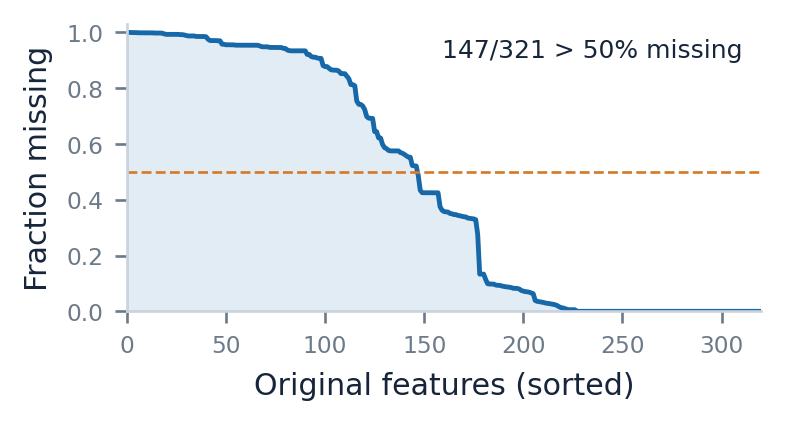
\includegraphics[width=\columnwidth]{missing_report}
\caption{Missing-value fraction among the 321 original features. The 147 variables above 50\% missing motivate fit-on-train filtering and explicit missing indicators. Coded nonresponses are not counted as NaN here.}
\label{fig:missing}
\end{figure}

\section{Model and Training}
Let $y_i\in\{0,1\}$ be the recoded labels. For encoded inputs $x_i$ we minimize
\begin{equation}
\label{eq:loss}
\frac1n\sum_{i=1}^n \left[\log(1+e^{x_i^\top w})-y_ix_i^\top w\right]
+\lambda\sum_{j\ge1}w_j^2.
\end{equation}
We optimize this logistic objective with an original NumPy mini-batch Adam implementation (batch size 8,192; learning rate 0.03; $\lambda=2\cdot10^{-4}$). The intercept is not regularized. Training runs for up to 12 epochs; the epoch with the lowest tuning-set cross-entropy is retained, with early stopping after four unimproved epochs.

\section{Evaluation Protocol}
We use stratified splits of 70\% training, 15\% tuning and 15\% evaluation data, with random seeds 42, 123 and 2026. Each split learns its encoder and weights only on training examples. The tuning partition selects the stopping epoch and an F1-maximizing decision threshold among $\{0.08,0.085,\dots,0.60\}$. The evaluation partition is never used for fitting the parameters or threshold. Comparing model variants on these partitions is exploratory model selection, so the reported scores should not be described as a final untouched estimate after all experiments. AIcrowd provides an additional held-out comparison.

\section{Experiments and Results}
\begin{table}[t]
\centering\caption{Positive-class F1 on evaluation partitions. Means $\pm$ sample SD across three stratified seeds. Clinical is from seed 42 only.}
\label{tab:abl}
\begin{tabular}{@{}lcc@{}}
\toprule
Feature set & Evaluation F1 & Splits \\
\midrule
Clinical, coded & 0.4311 & 1 \\
Encoded, no interactions & $\mathbf{0.4324\pm0.0032}$ & 3 \\
Encoded + 7 interactions & $0.4324\pm0.0024$ & 3 \\
\bottomrule
\end{tabular}
\end{table}
The interaction set provides no repeatable improvement: the mean paired difference (with minus without) is $-0.00005$ F1 across the three splits. We select the simpler encoded model for our final submission. The clinical baseline achieves 0.4311 on seed 42; the two encoded variants achieve 0.4339 and 0.4342 on the same seed, respectively.

\subsection{Why the threshold matters}
On seed 42, tuning selects $t=0.230$ and six epochs (Fig.~\ref{fig:threshold}). At this \emph{locked} threshold, the held-out partition gives accuracy 0.8761, precision 0.3637, recall 0.5375 and F1 0.4339. The conventional cutoff $t=0.5$ yields F1 0.2525 on that same partition. The confusion matrix is $\mathrm{TP}=2,336$, $\mathrm{FP}=4,086$, $\mathrm{FN}=2,010$, $\mathrm{TN}=40,788$.

\begin{figure}[t]
\centering
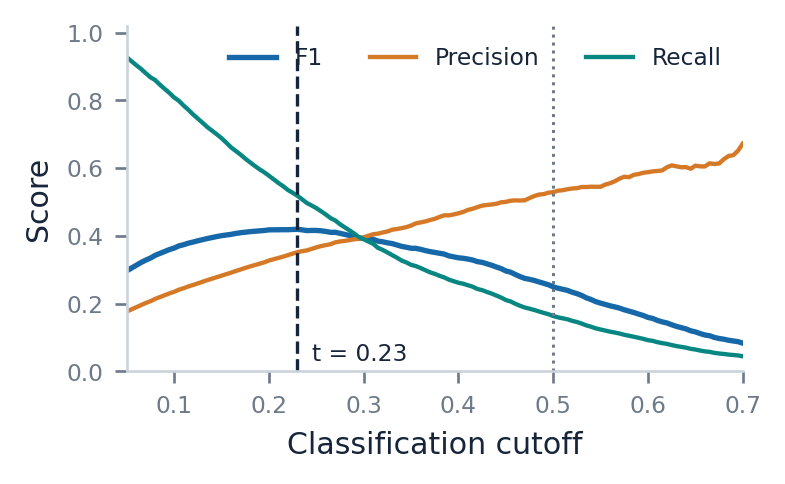
\includegraphics[width=\columnwidth]{threshold_report}
\caption{F1, precision and recall as functions of the decision threshold on the \emph{tuning} partition (seed 42). Dashed line: chosen $t=0.230$ on tuning rows. The held-out evaluation set is not searched for a threshold.}
\label{fig:threshold}
\end{figure}

\subsection{Competition result}
A final NumPy logistic model was fitted using all labeled data, with the epoch count and classification cutoff selected beforehand on the local validation split. The uploaded AIcrowd CSV (submission \#338016, 27 October 2026) obtained \textbf{F1 = 0.436} and accuracy = 0.870. This agreement with local validation is encouraging, but not proof of clinical generalizability.

\section{Discussion and Conclusion}
Survey response coding and the classification threshold influence F1 much more than adding our seven interaction terms. Some fitted weights align with intuitive associations (e.g., stroke history and poorer health correlate with a positive prediction), but coefficients of one-hot-encoded, correlated survey variables are not causal effects. The data are self-reported and cross-sectional, and the prevalence is imbalanced. The principal contribution is a reproducible NumPy-only pipeline with separate tuning and evaluation partitions, plus an ablation showing that a simpler representation can perform as well as the extended one.

\begin{figure}[t]
\centering
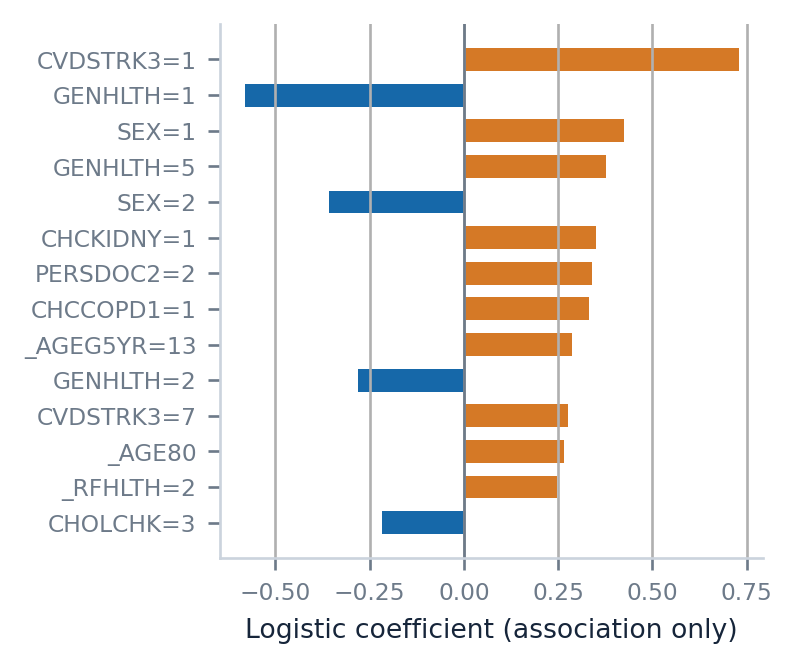
\includegraphics[width=\columnwidth]{weights_report}
\caption{Largest absolute coefficients on training seed 42, after one-hot encoding and L2 regularization. The sign is coding-dependent and must not be read causally.}
\label{fig:weights}
\end{figure}

\section{Error Analysis and Reproducibility}
On the seed-42 evaluation partition, the model flags 6,422 individuals as positive: 2,336 true positives versus 4,086 false positives. It misses 2,010 positives. Although the F1-optimized threshold increases sensitivity compared with 0.5, more than half of its positive predictions are false alarms (precision 36.37\%). For medical deployment, calibration, external validation and a well-defined cost for missed cases versus false alarms would be essential. The observations also do not justify any causal interpretation of individual encoded weights (Fig.~\ref{fig:weights}).

All reported local experiments use the provided dataset and deterministic random seeds. Training features are fitted within each training partition; epochs and thresholds come from the tuning partition. The figure generator stores per-seed ablation results in \texttt{documentation/ziyad\_results.json}, retrains the seed-42 diagnostic model, and writes all plots. Running it with \texttt{--recompute-ablation} independently retrains both ablation variants across all three seeds. The competition submission is produced by \texttt{submissions/ziyad.py} using \texttt{--mode submit}, \texttt{--features expanded\_no\_interactions}, \texttt{--epochs 12}, \texttt{--l2 0.0002}, and \texttt{--optimize f1}.
\end{document}
